\part{Neural Networks}
%%%%%%%%%%%%%%%%%%%%%%%%%%%%%%%%%%%%%%%%%%%%%%%%%%%%%%%%%%%%%%%%%%%%%%%%%
% Intel Neural Compute Stick 2                                          %
%%%%%%%%%%%%%%%%%%%%%%%%%%%%%%%%%%%%%%%%%%%%%%%%%%%%%%%%%%%%%%%%%%%%%%%%%
\section{Motivation and background}
The motivation of this project is a logical continuation of part 4 with the Intel Realsense Camera. In the previous project, a Hardkernal Odroid XU4 was used because it is comparitevly cheaper than existing hardware used for Surewash products, the issue is that this is still comparitevly expensive in comparison to a Raspberry Pi (a casual search on Amazon suggests that it is at least 3-4 times more expensive). The issue with the Raspberry Pi is that its hardware is not capable of running the Surewash algorithm in a time critical setting, which is of course needed, since one of the key selling points of Surewash is that it can give live feedback to the user. A potential solution to this problem is using an Intel Neural Compute Stick, hereafter NCS. This is a low-power device that can interface with a Raspberry Pi via the USB protocol. The cornerstone of the NCS is the Myriad chip.

The Myriad chip is described by Intel as a 'Vision Processing Unit', hereafter VPU (not to be confused with a Video Processing Unit). One might already be familiar with the concept of a CPU, or Central Processing Unit, which is a microchip designed for general purpose computing, and a GPU, or Graphics Processing Unit, which is specifically optimised for {\slshape embarrassingly parallel} calculations, such as graphics processing, hence the name. The VPU is similar in idea to a GPU in that it is optimised for parallel computing, except that it is specifically designed for low-power situations \cite{7024073}, and it is particularly suited for inferring convolutional and fully-connected neural networks on mobile devices.

The current Surewash algorithm uses traditional computer vision methods which are not well suited for a device like the NCS, and so the algorithm for processing hand gestures will have to be completely rethought in order to work on the NCS.

\section{Underlying concepts}
    \subsection{Graphs}
    A graph is a is a mathematical concept where a series of nodes are connected together by vertices \cite{chartrand2010graphs}. A classical example of graph theory theory in the real world would be for computer-aided map directions, locations can be nodes, and roads vertices. A computer could give directions based on this graph using {\slshape Dijkstra's Algorithm} \cite{dijkstra1959note}.

    \begin{figure}[h]
        \centering
        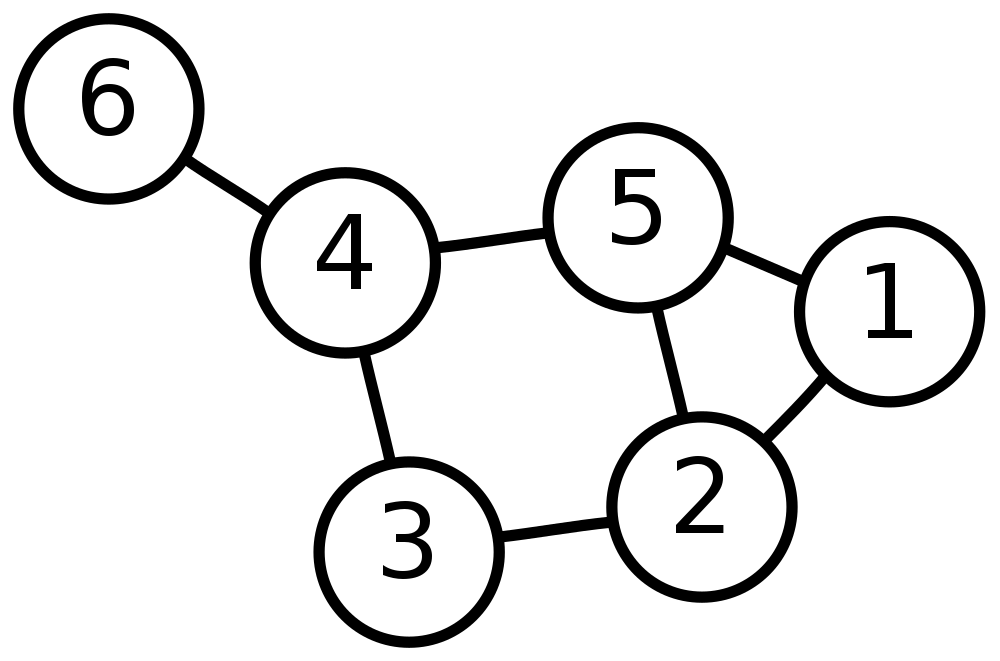
\includegraphics[width=100px]{../img/1000px-6n-graf.png}
        \caption{Obtained from: https://commons.wikimedia.org/wiki/File:6n-graf.svg (accessed: 26-05-2019)}
        \label{fig:simplegraph}
    \end{figure}

    Figure \ref{fig:simplegraph} is an example of a simple graph. Graphs can be broken down into two broad types: undirected, and directed. In an undirected graph, the vertices are always unidirectional, but in a directed graph, or digraph, each vertex in a graph has a direction associated with it. In a graph, the vertices can also have weights associated with them. For example, in the context of a graph to model a road map, larger weights might denote a longer road, and a smaller weight, a shorter road. The graph is the fundamental building block to Artificial Neural Networks.

    \subsection{Artificial Neural Networks}
    Artificial Neural Networks, hereafter ANNs in essecence are graphs. Specifically, ANNs are directed, acyclic, weighted graphs. An acyclic graph is one that has a defined entry and exit point, and no loops with in the graph, so the evaluation of the graph is finite. ANN are so-called because they aim to emulate the function of Biological Neural Networks, so each node acts as a 'neuron', with defined weighted connections to other neurons \cite{hopfield1982neural}. In a typical ANN, neurons are divided into a sequence of layers starting with the input layer, then one or more 'hidden' layers, followed by an output layer. Each neuron in a layer is connected some or all neurons in the previous layer with weighted vertices, its output is the sum of those weighted vertices passed into some function, called the activation function. 

    \begin{figure}[h]
        \centering
        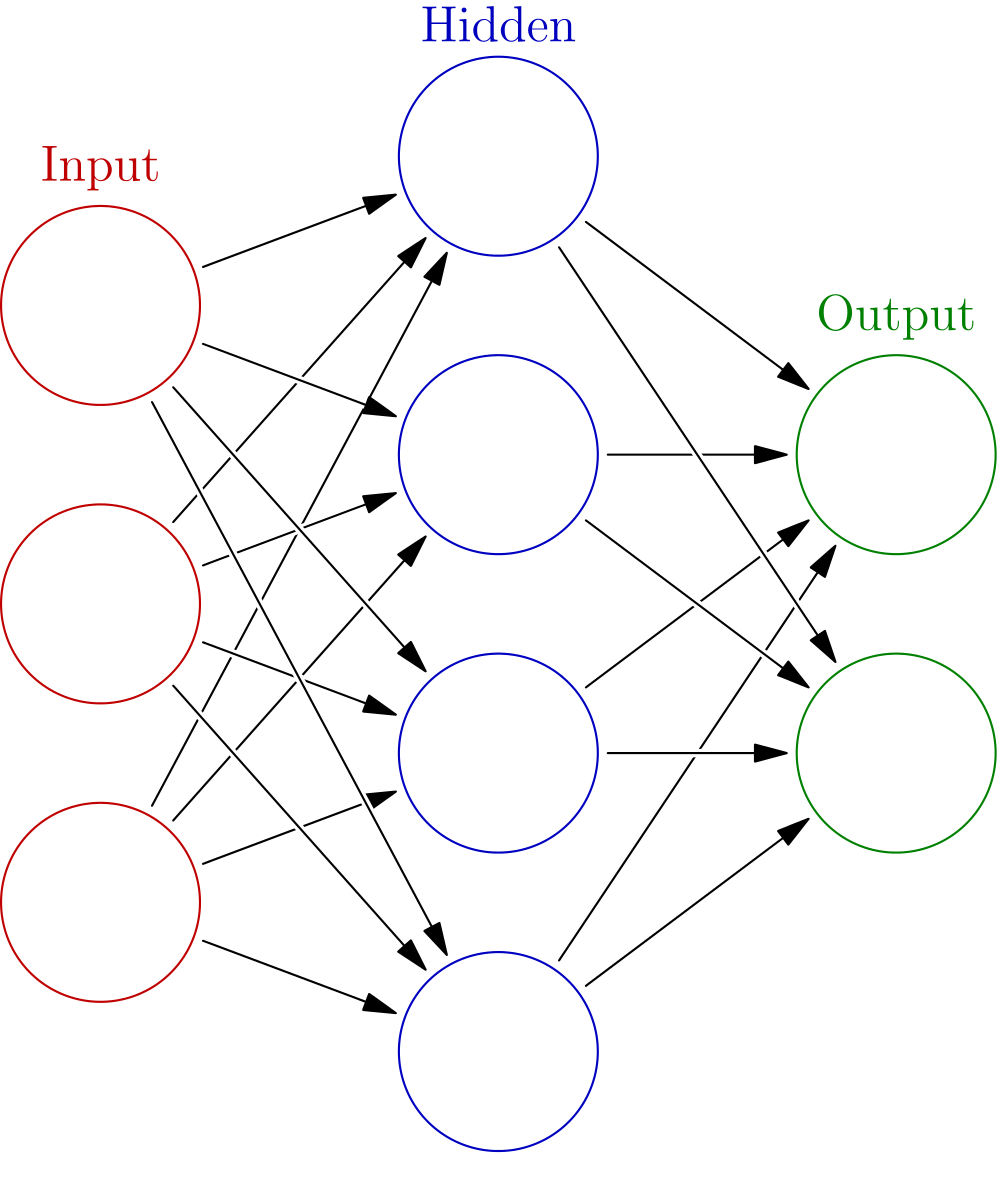
\includegraphics[width=150px]{../img/1000px-Colored_neural_network.png}
        \caption{Obtained from: https://commons.wikimedia.org/wiki/File:Colored\_neural\_network.svg (accessed: 26-05-2019) \copyright \space Glosser.ca, available under a CC BY-SA 3.0 license \url{https://creativecommons.org/licenses/by-sa/3.0/deed.en}}
        \label{fig:fcneuralnet}
    \end{figure}

    Figure \ref{fig:fcneuralnet} is an example of a simple neural network (the neurons are 'fully connected', so each neuron in a layer is connected to all of the neurons from the previous layer), this graph takes three scalar inputs, and produces two scalar outputs.

        \subsubsection{The Neuron}
        Formally, a neuron looks like Figure \ref{fig:theneuron}.
        \begin{figure}[h]
        \[
            u=f(w_0+\sum_{i=1}^nw_ix_i)
        \]
        \caption{The Nueron}
        \label{fig:theneuron}
        \end{figure}
        Where $x_i$ represents the input of a previous neuron, or the entry to the graph, $w_i$ represents a weight that $x_i$ is multiplied by, $w_0$ represents the 'bias' which is simply a scalar value, and $f$ is some function that produces a scalar output for that neuron.
        
        \subsubsection{Activation Functions}

        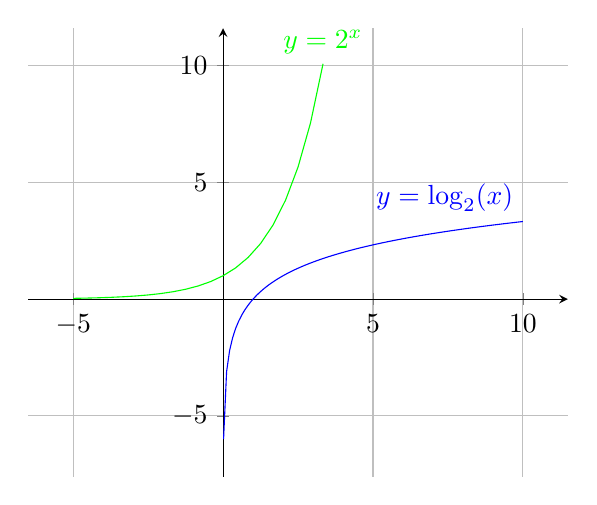
\begin{tikzpicture}
            \begin{axis}[grid=both,
                xmax=10,ymax=10,
                axis lines=middle,
                restrict y to domain=-7:12,
                enlargelimits]
            \addplot[green]  {pow(2,x)} node[above]{$y=2^x$};
            \addplot[blue,domain=1/2^6:10,samples=100]  {log2(x)} node[above left] {$y=\log_2(x)$};
            \end{axis}
          \end{tikzpicture}

          \subsubsection{Training ANNs}
          {\slshape Insert stuff about the loss function and back propagation}
    
    \section{Workflow}
        \subsection{Hardware}
        Training a neural network is not a trivial task computationally speaking. The computer that I work with, by today's standards has a high specification, but it is wholly inadequate for training neural networks, which is due to the nature of how neural networks are trained. Graphics Processing Units, or GPUs have been shown to be quicker at training neural networks \cite{OH20041311}. Since there was no adequate GPU readily available at work, I set up an AWS instance which had a GPU. I did have to be concious of cost, since the the server cost circa USD\$0.80 per hour and my budget was limited. As an example of the differance that using AWS makes, I compared training the same neural network on my computer, and on AWS, to train one epoch on my own computer took approximately 60 minutes, but only took 2 minutes on AWS.

        Any work that did not involve training neural networks was completed on my own computer.

        \subsection{Software}
            \subsubsection{Programming Language}
            Most programming was done with the Intel distribution of Python (my own computer has an Intel Coffee Lake CPU) since it is compiled to take advantage of CPU instructions for vector manipulation. Some miscellaneous work was also done with Bash script.

            \subsubsection{ANN Training}
            For designing and training the neural networks, I used Keras \cite{chollet2015keras} because I had used it before. Keras is a high-level Python framework for designing ANNs, and acts for a frontend for other ANN franeworks, I choose Tensorflow \cite{tensorflow2015-whitepaper} as the backend because it is compatible with the NCS, and it is also relatively ubiquitous among the deep learning community.

            \subsubsection{Miscellaneous Processing}
            Numpy is a Python library for fast matrix multiplication. Since Python is a scripted language, vector and matrix operations are slow in native code, so Numpy can process these operations faster.

    \section{Data}
        \subsection{Introduction}
        As of writing this, it is still something of an open question as to how much data is required to effectively train a neural network, one of the key challenges with this project is aquiring enough data. When I started the project, I was given a labelled dataset containing 5114 images of hands, which is certainly too small, when ANNs such as VGG16 \cite{vggnet} were trained on many multiples the size of the dataset that I was given. The simplest strategy is to aquire more data, but without a defined procedure in place, this can be a time consuming, and costly process. Another strategy to get around limited data is employ data augmentation, such as rotations, affine transformations, and background modification.

        \subsection{Data Aquisition}
        Aquiring more data is the best way to overcome a small dataset, but the aquisition process needs to be streamlined in order to acheive this task effectively. This was forked into a seperate project which is described in the next part.

        \subsection{Data Augmentation}
            \subsubsection{Backgrounds}
            The background for the dataset given was a white sheet, so if the ANN was trained on just this, it is unlikely to work with any other type of background. My strategy to ensure that the ANN learns to ignore the background, is inputting images of hands among a diverse range of backgrounds. A convenient aspect of the data that I was given was that each inmage of a hand pose contained a corresponding binary image seperating foreground and background pixels, it is therefore a trivial task to replace the background of these images.

            \[ Y_{foreground} = HAND \land ROI \]
            \[ Y_{background} = BACKGROUND \land \lnot ROI \]
            \[ OUTPUT = Y_{background} \lor Y_{foreground} \]

            \begin{figure}[h]
                \centering
                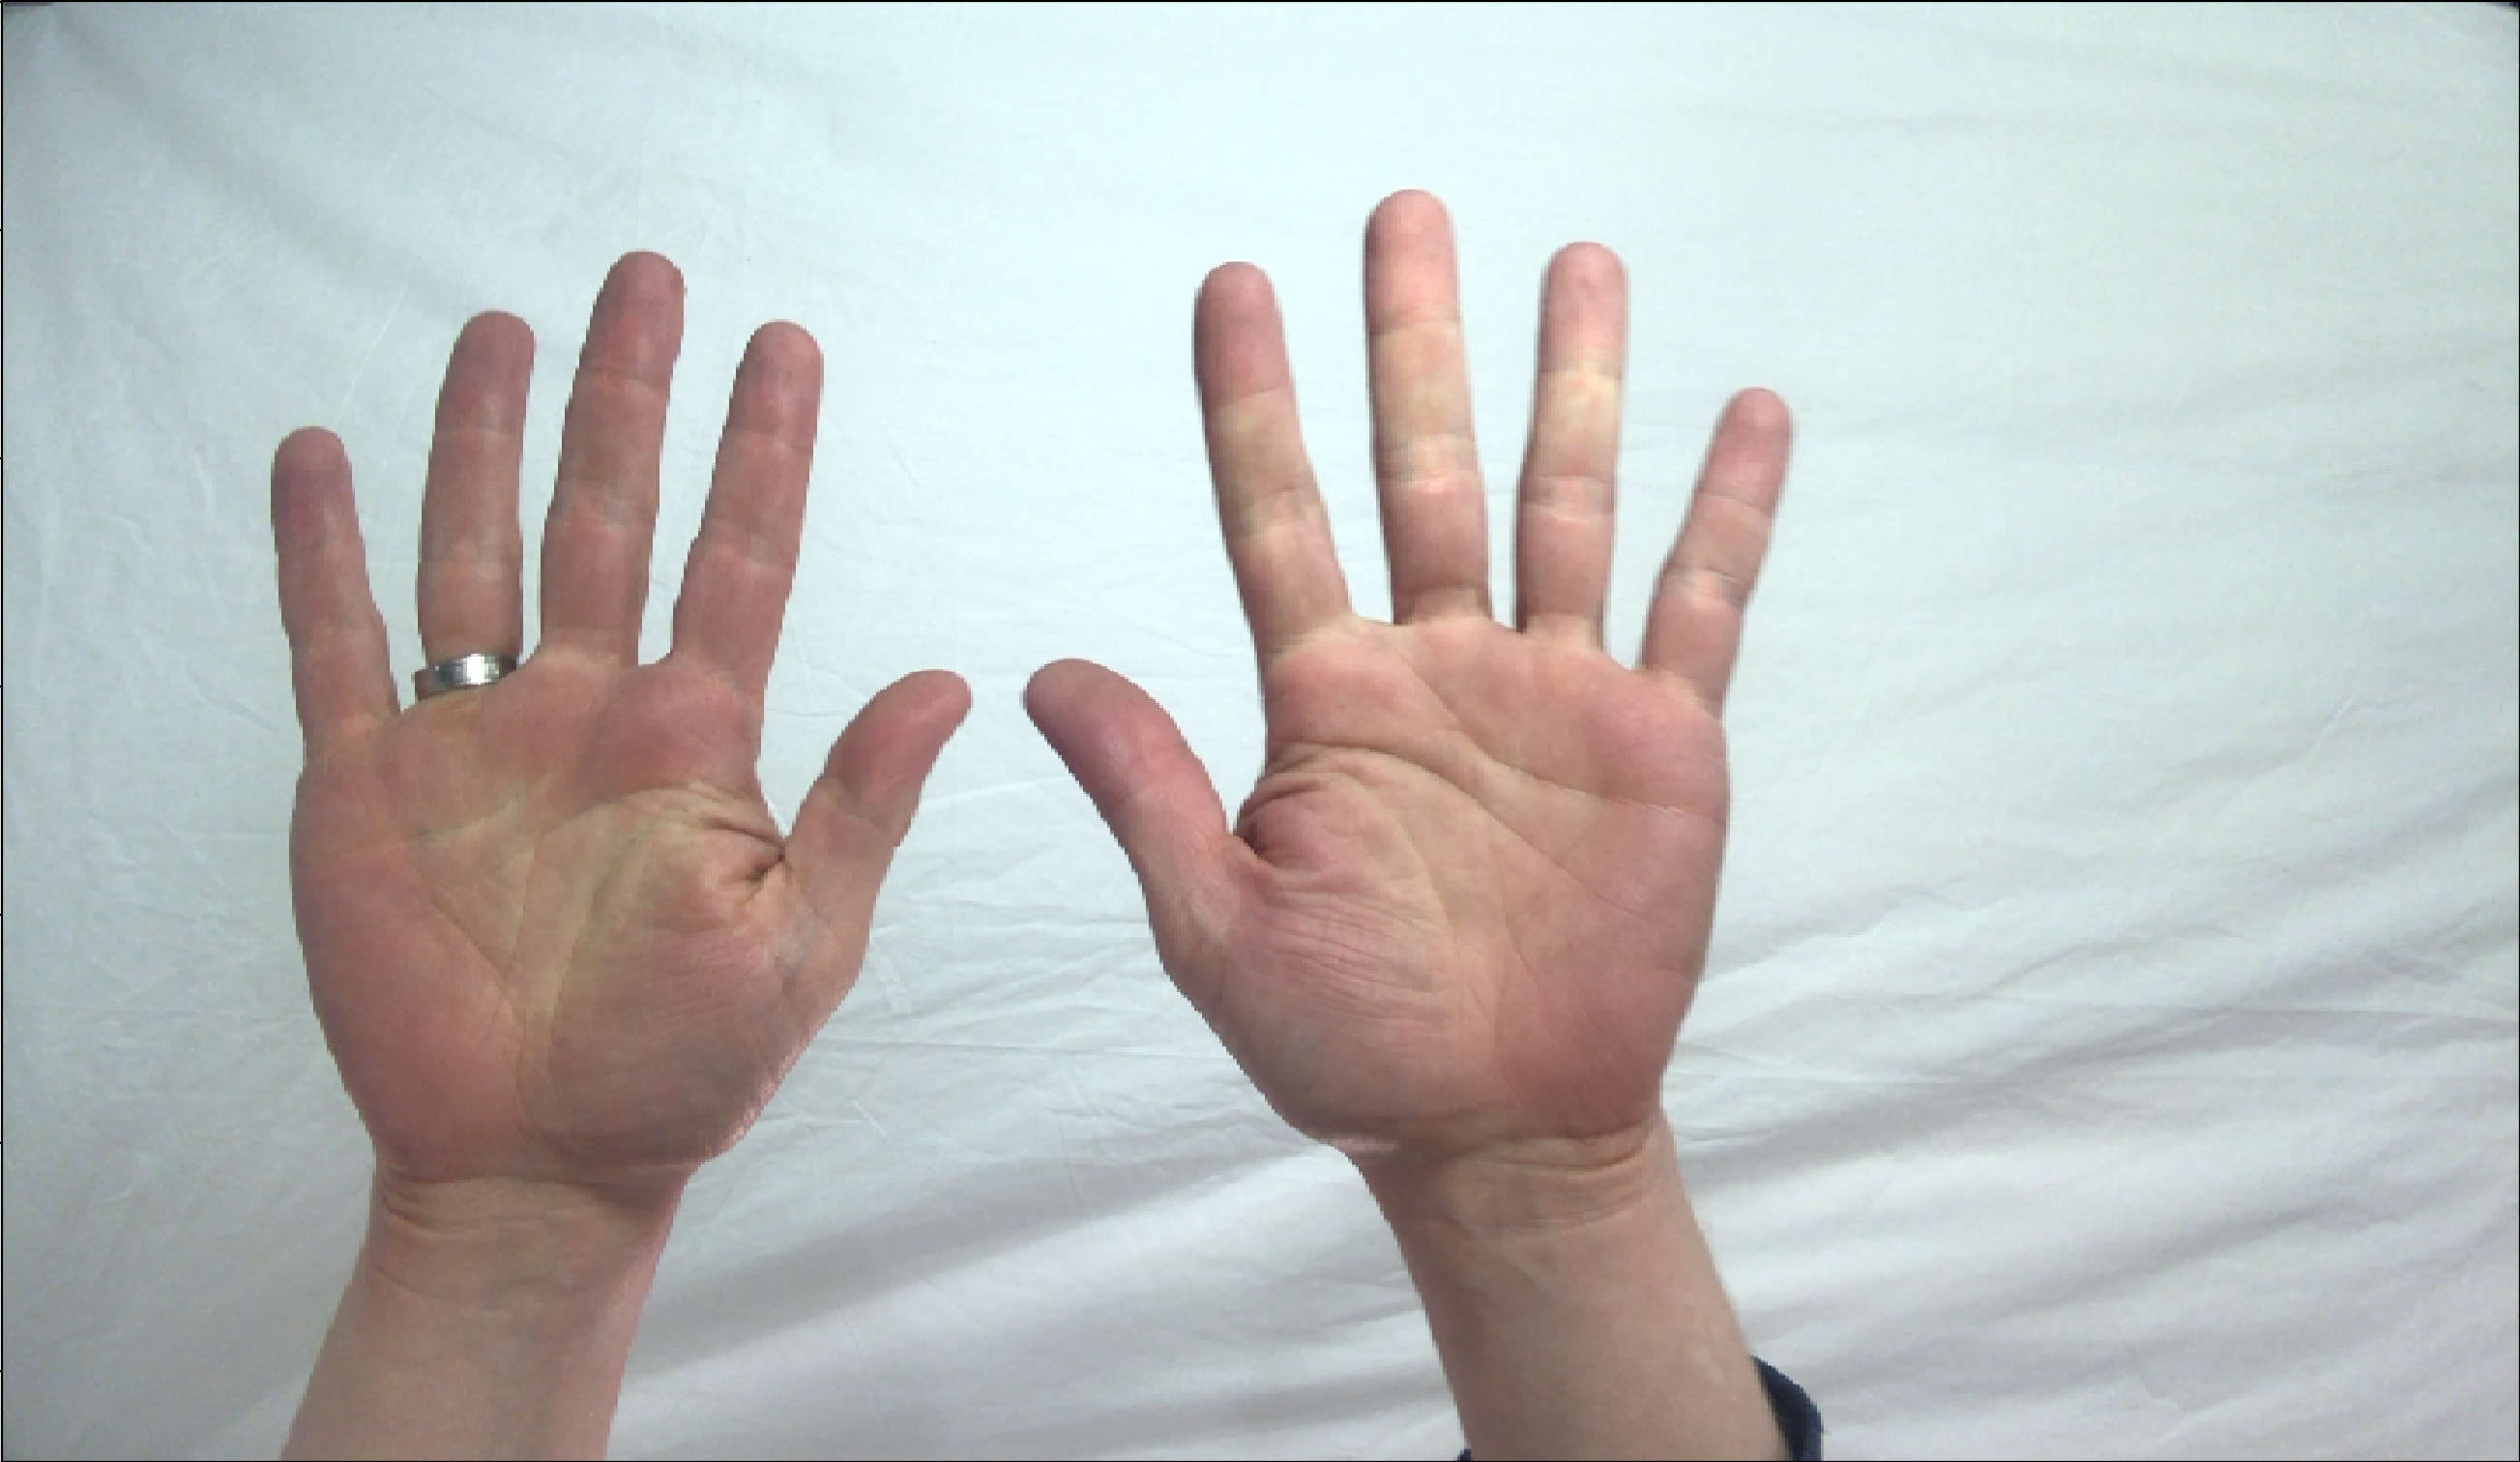
\includegraphics[width=114pt]{../img/handspipeline/1.png}
                
\includegraphics[width=114pt]{../img/handspipeline/2.png}
                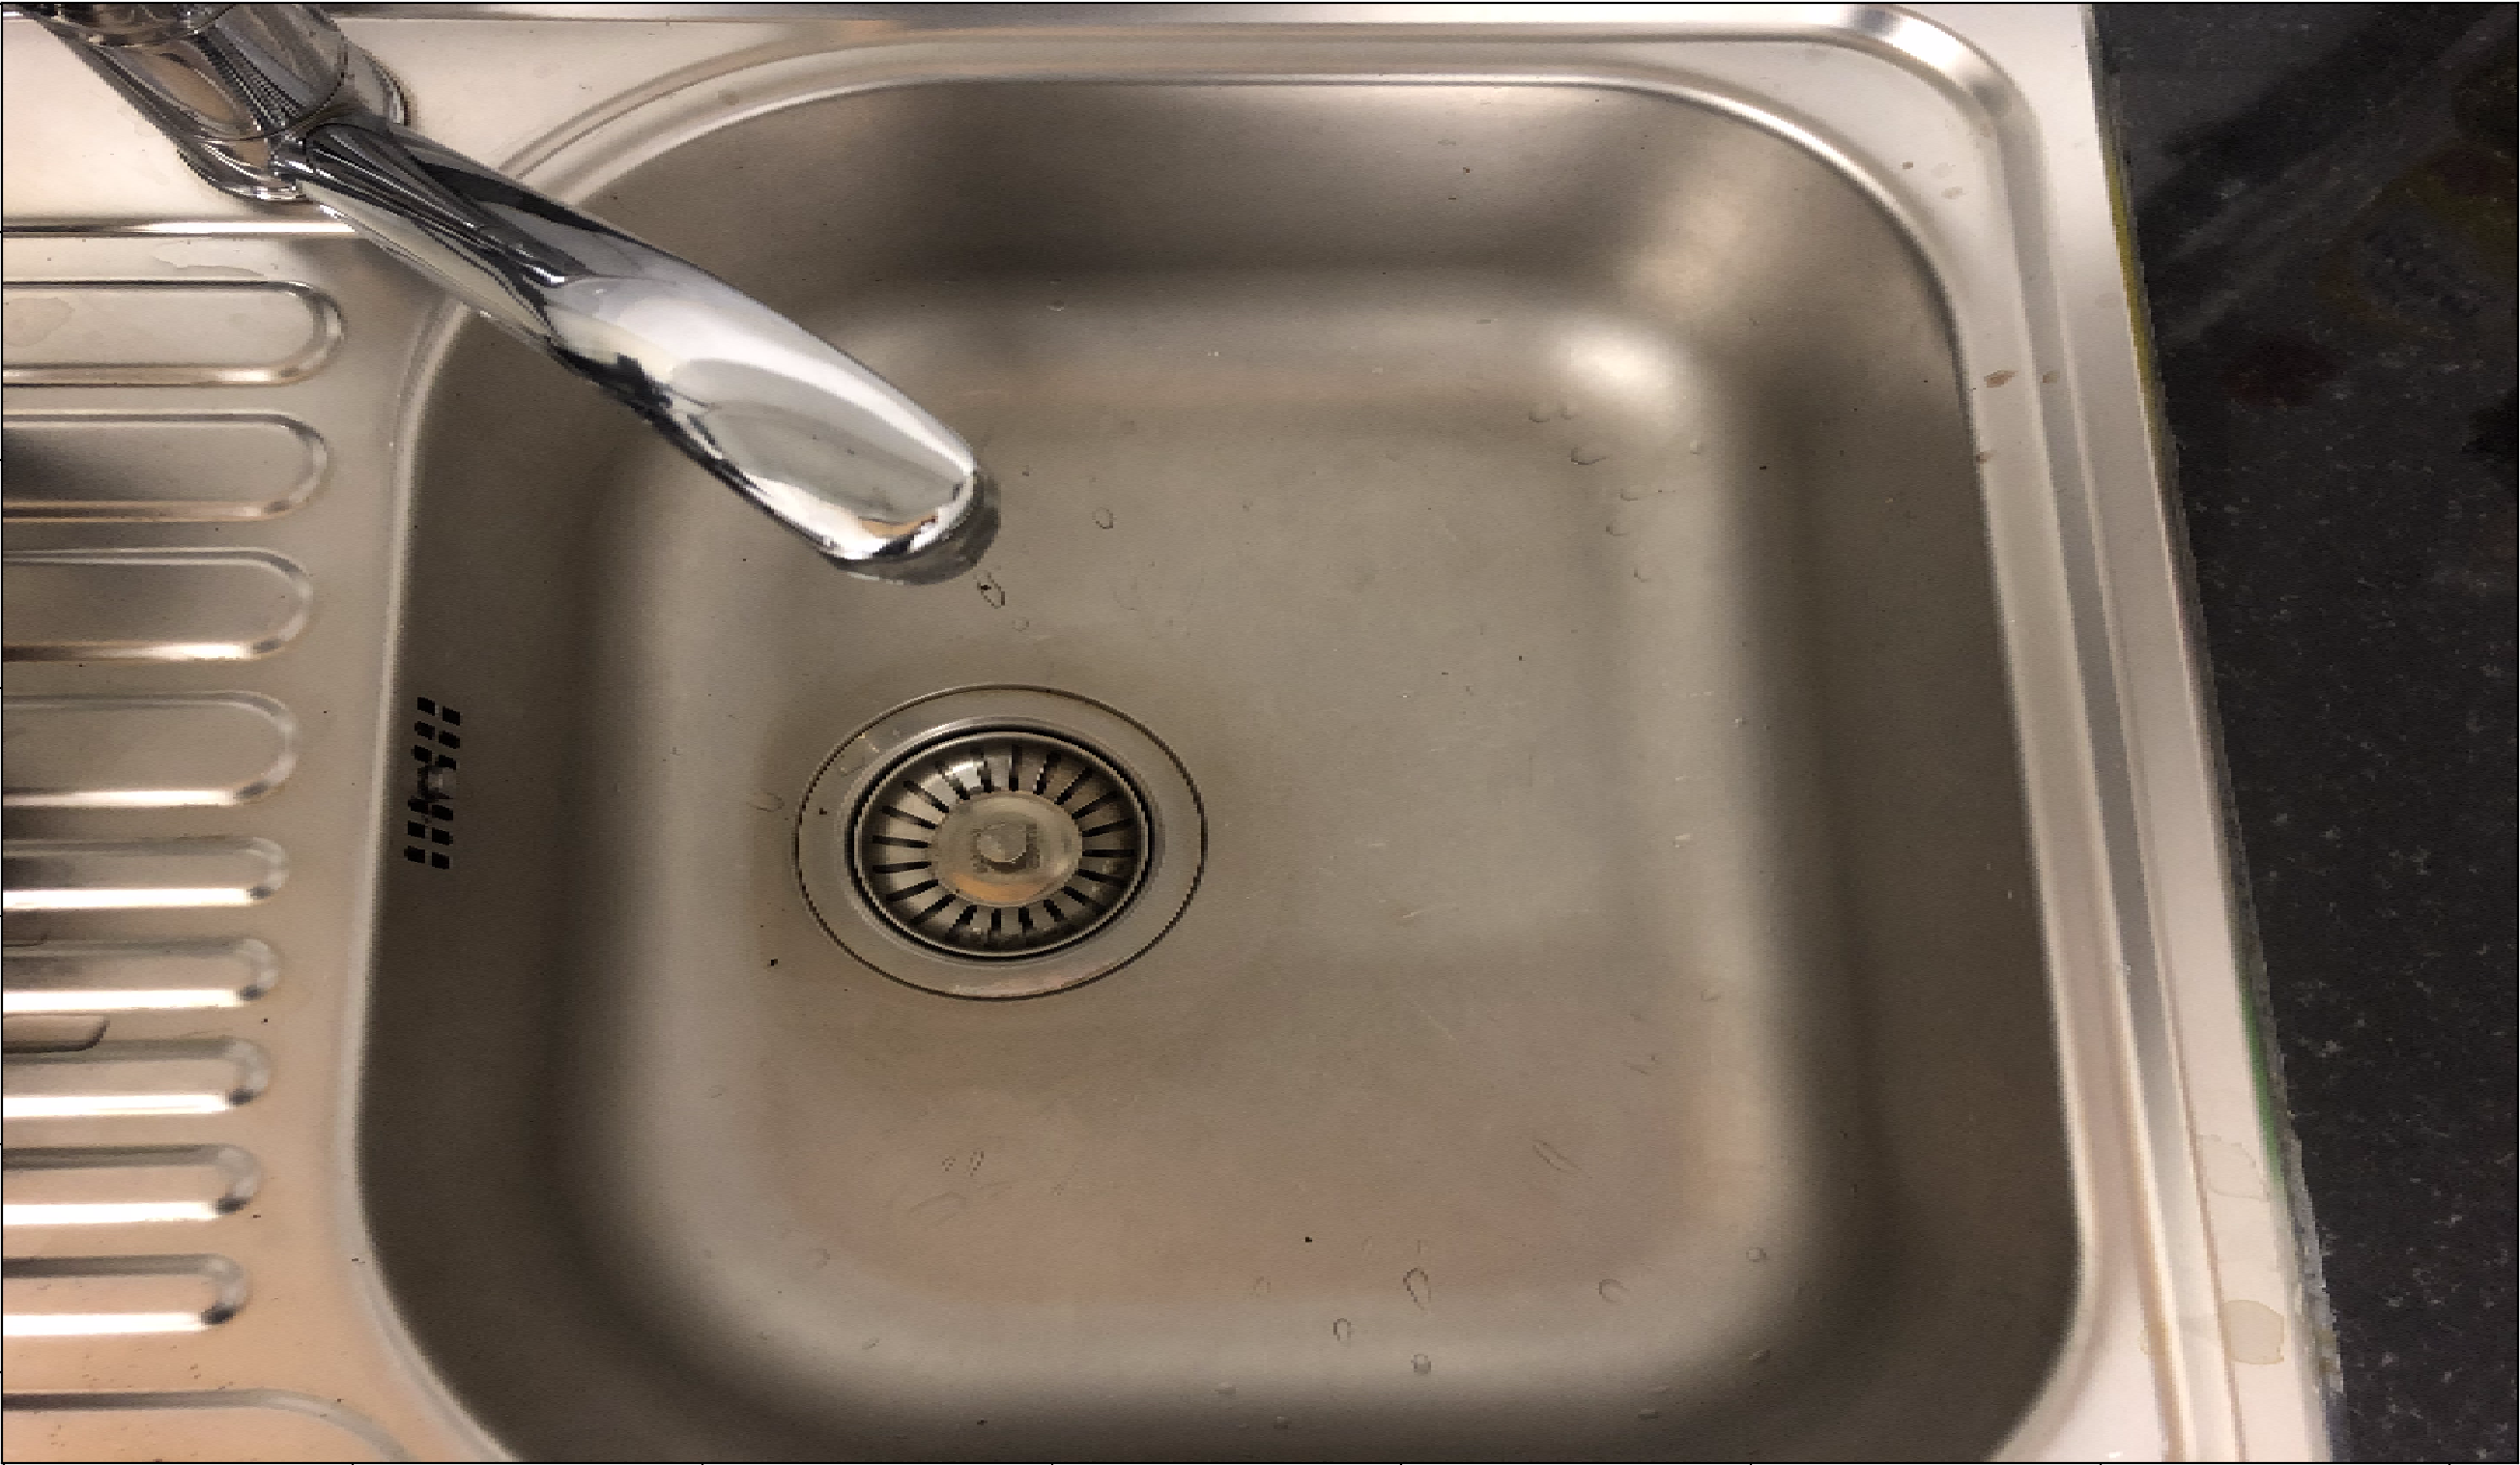
\includegraphics[width=114pt]{../img/handspipeline/3.png}\\
                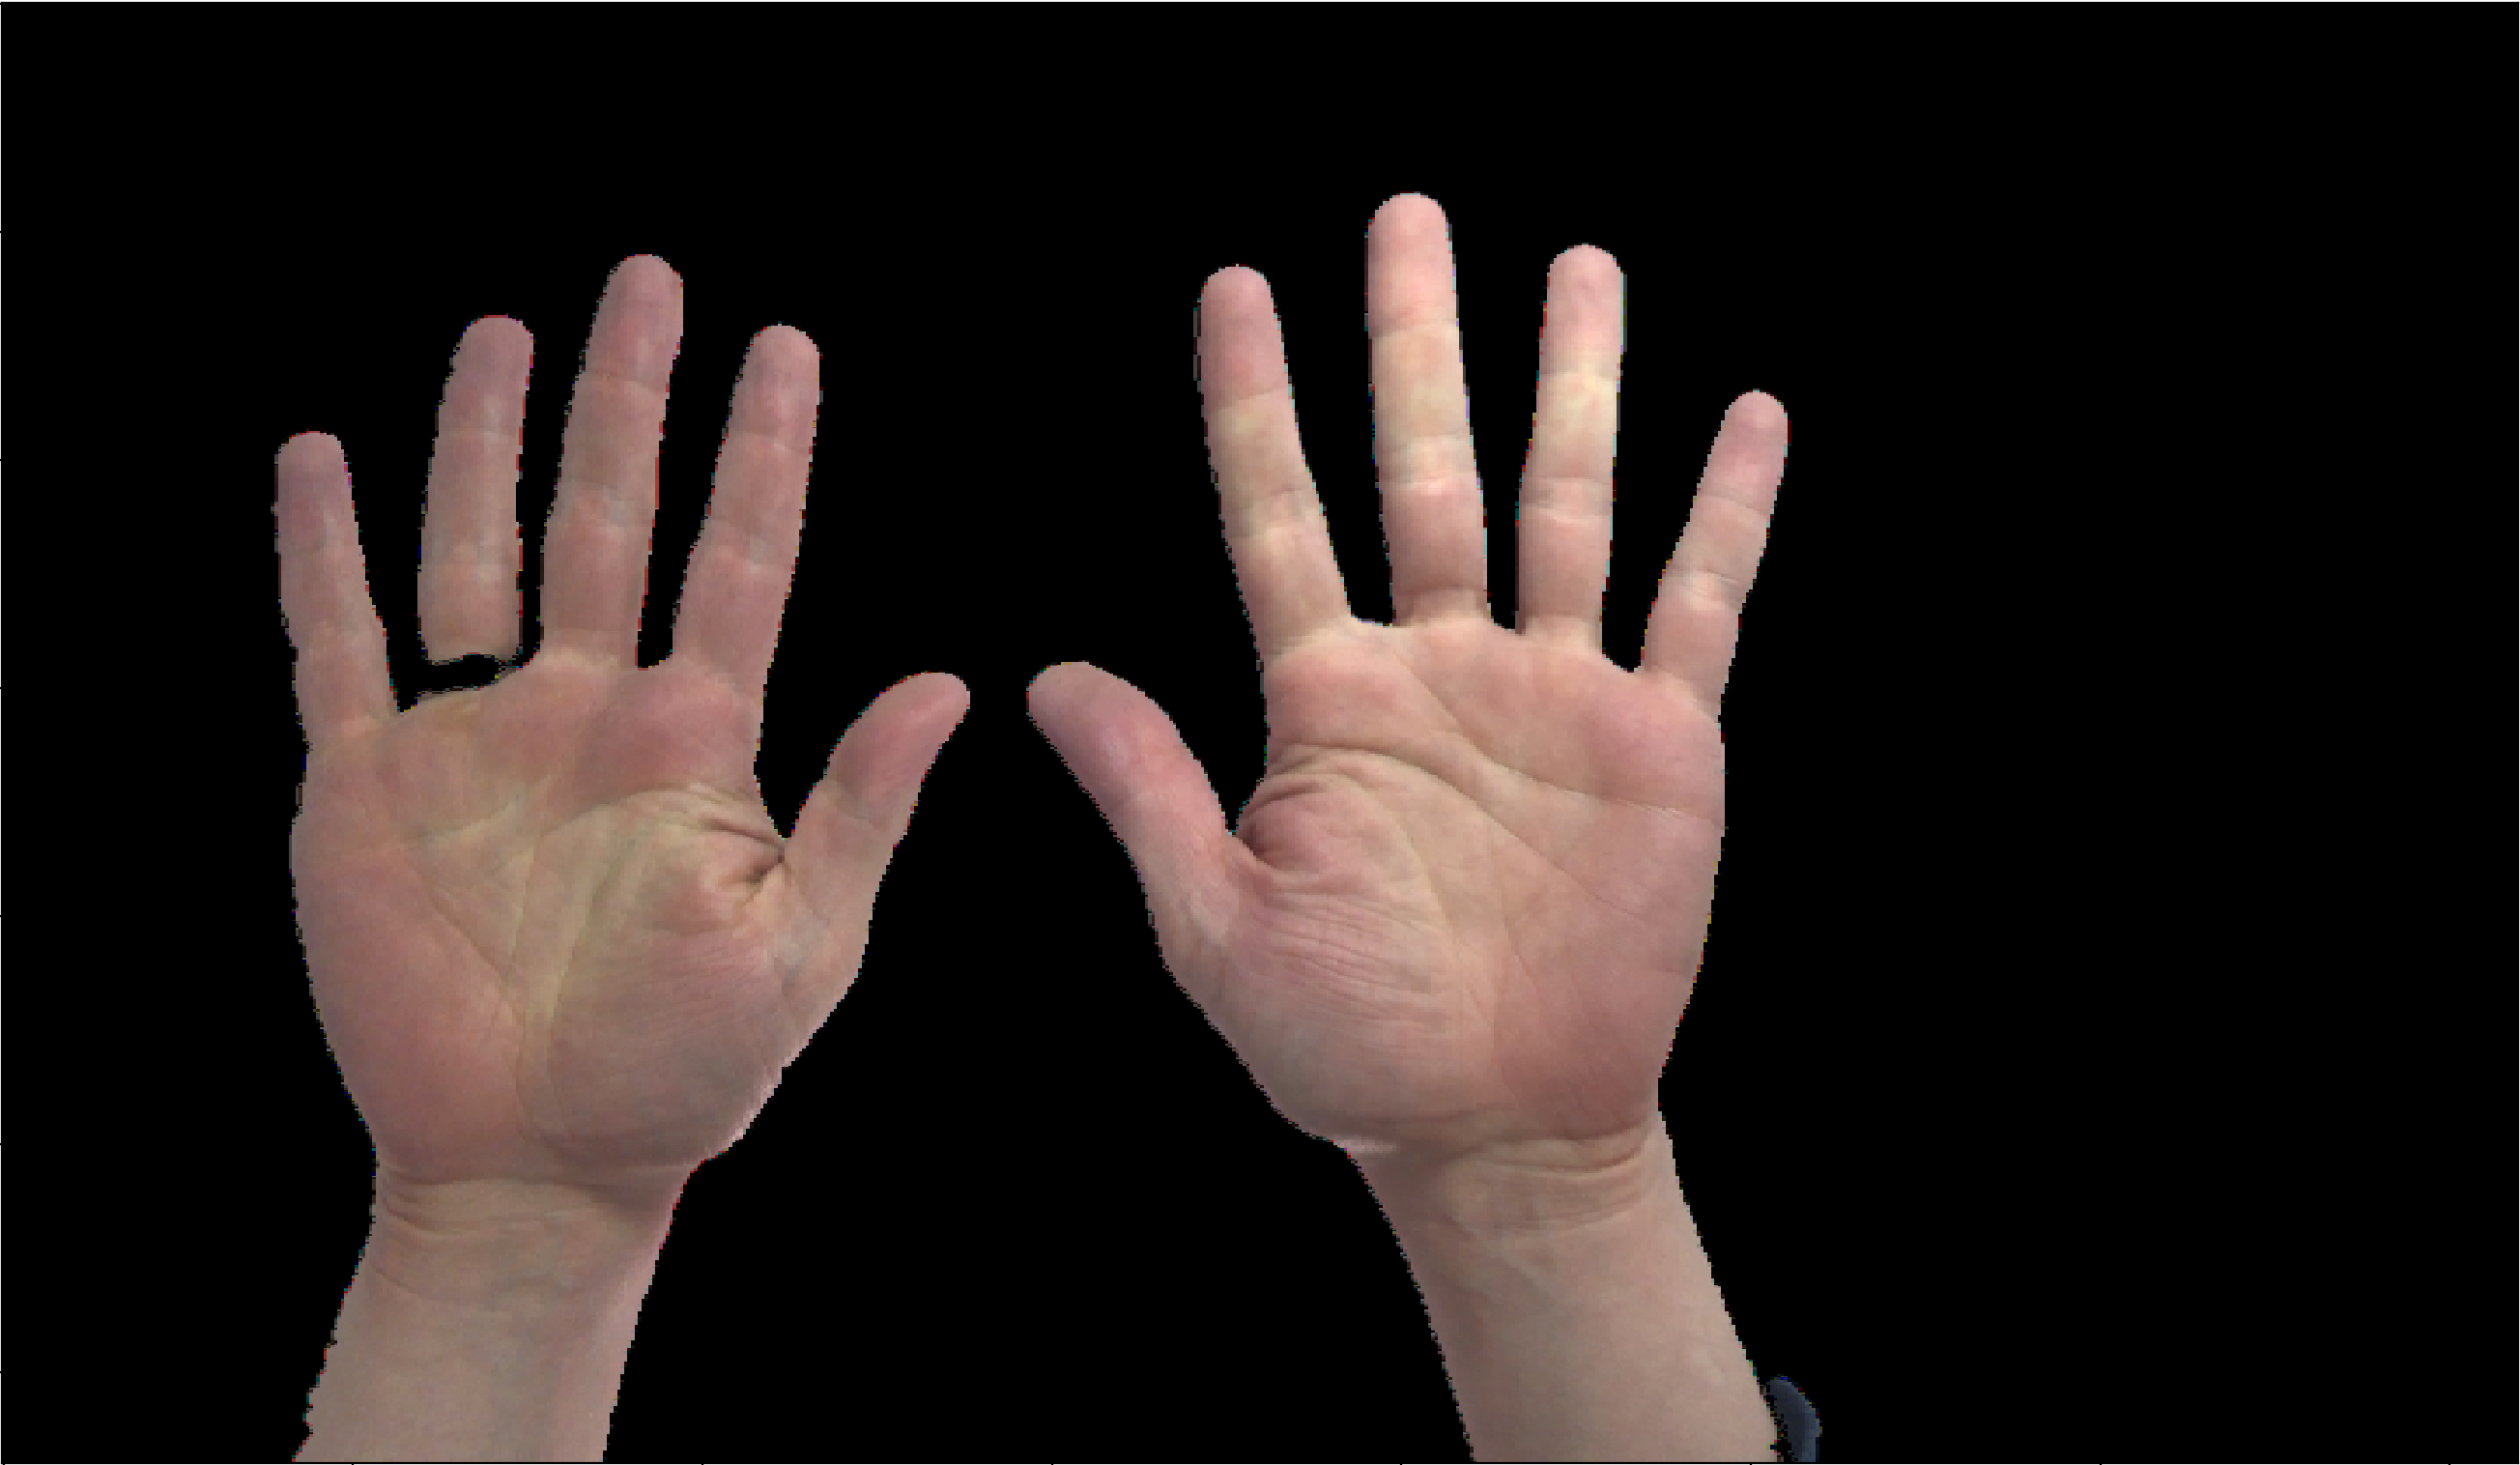
\includegraphics[width=114pt]{../img/handspipeline/4.png}
                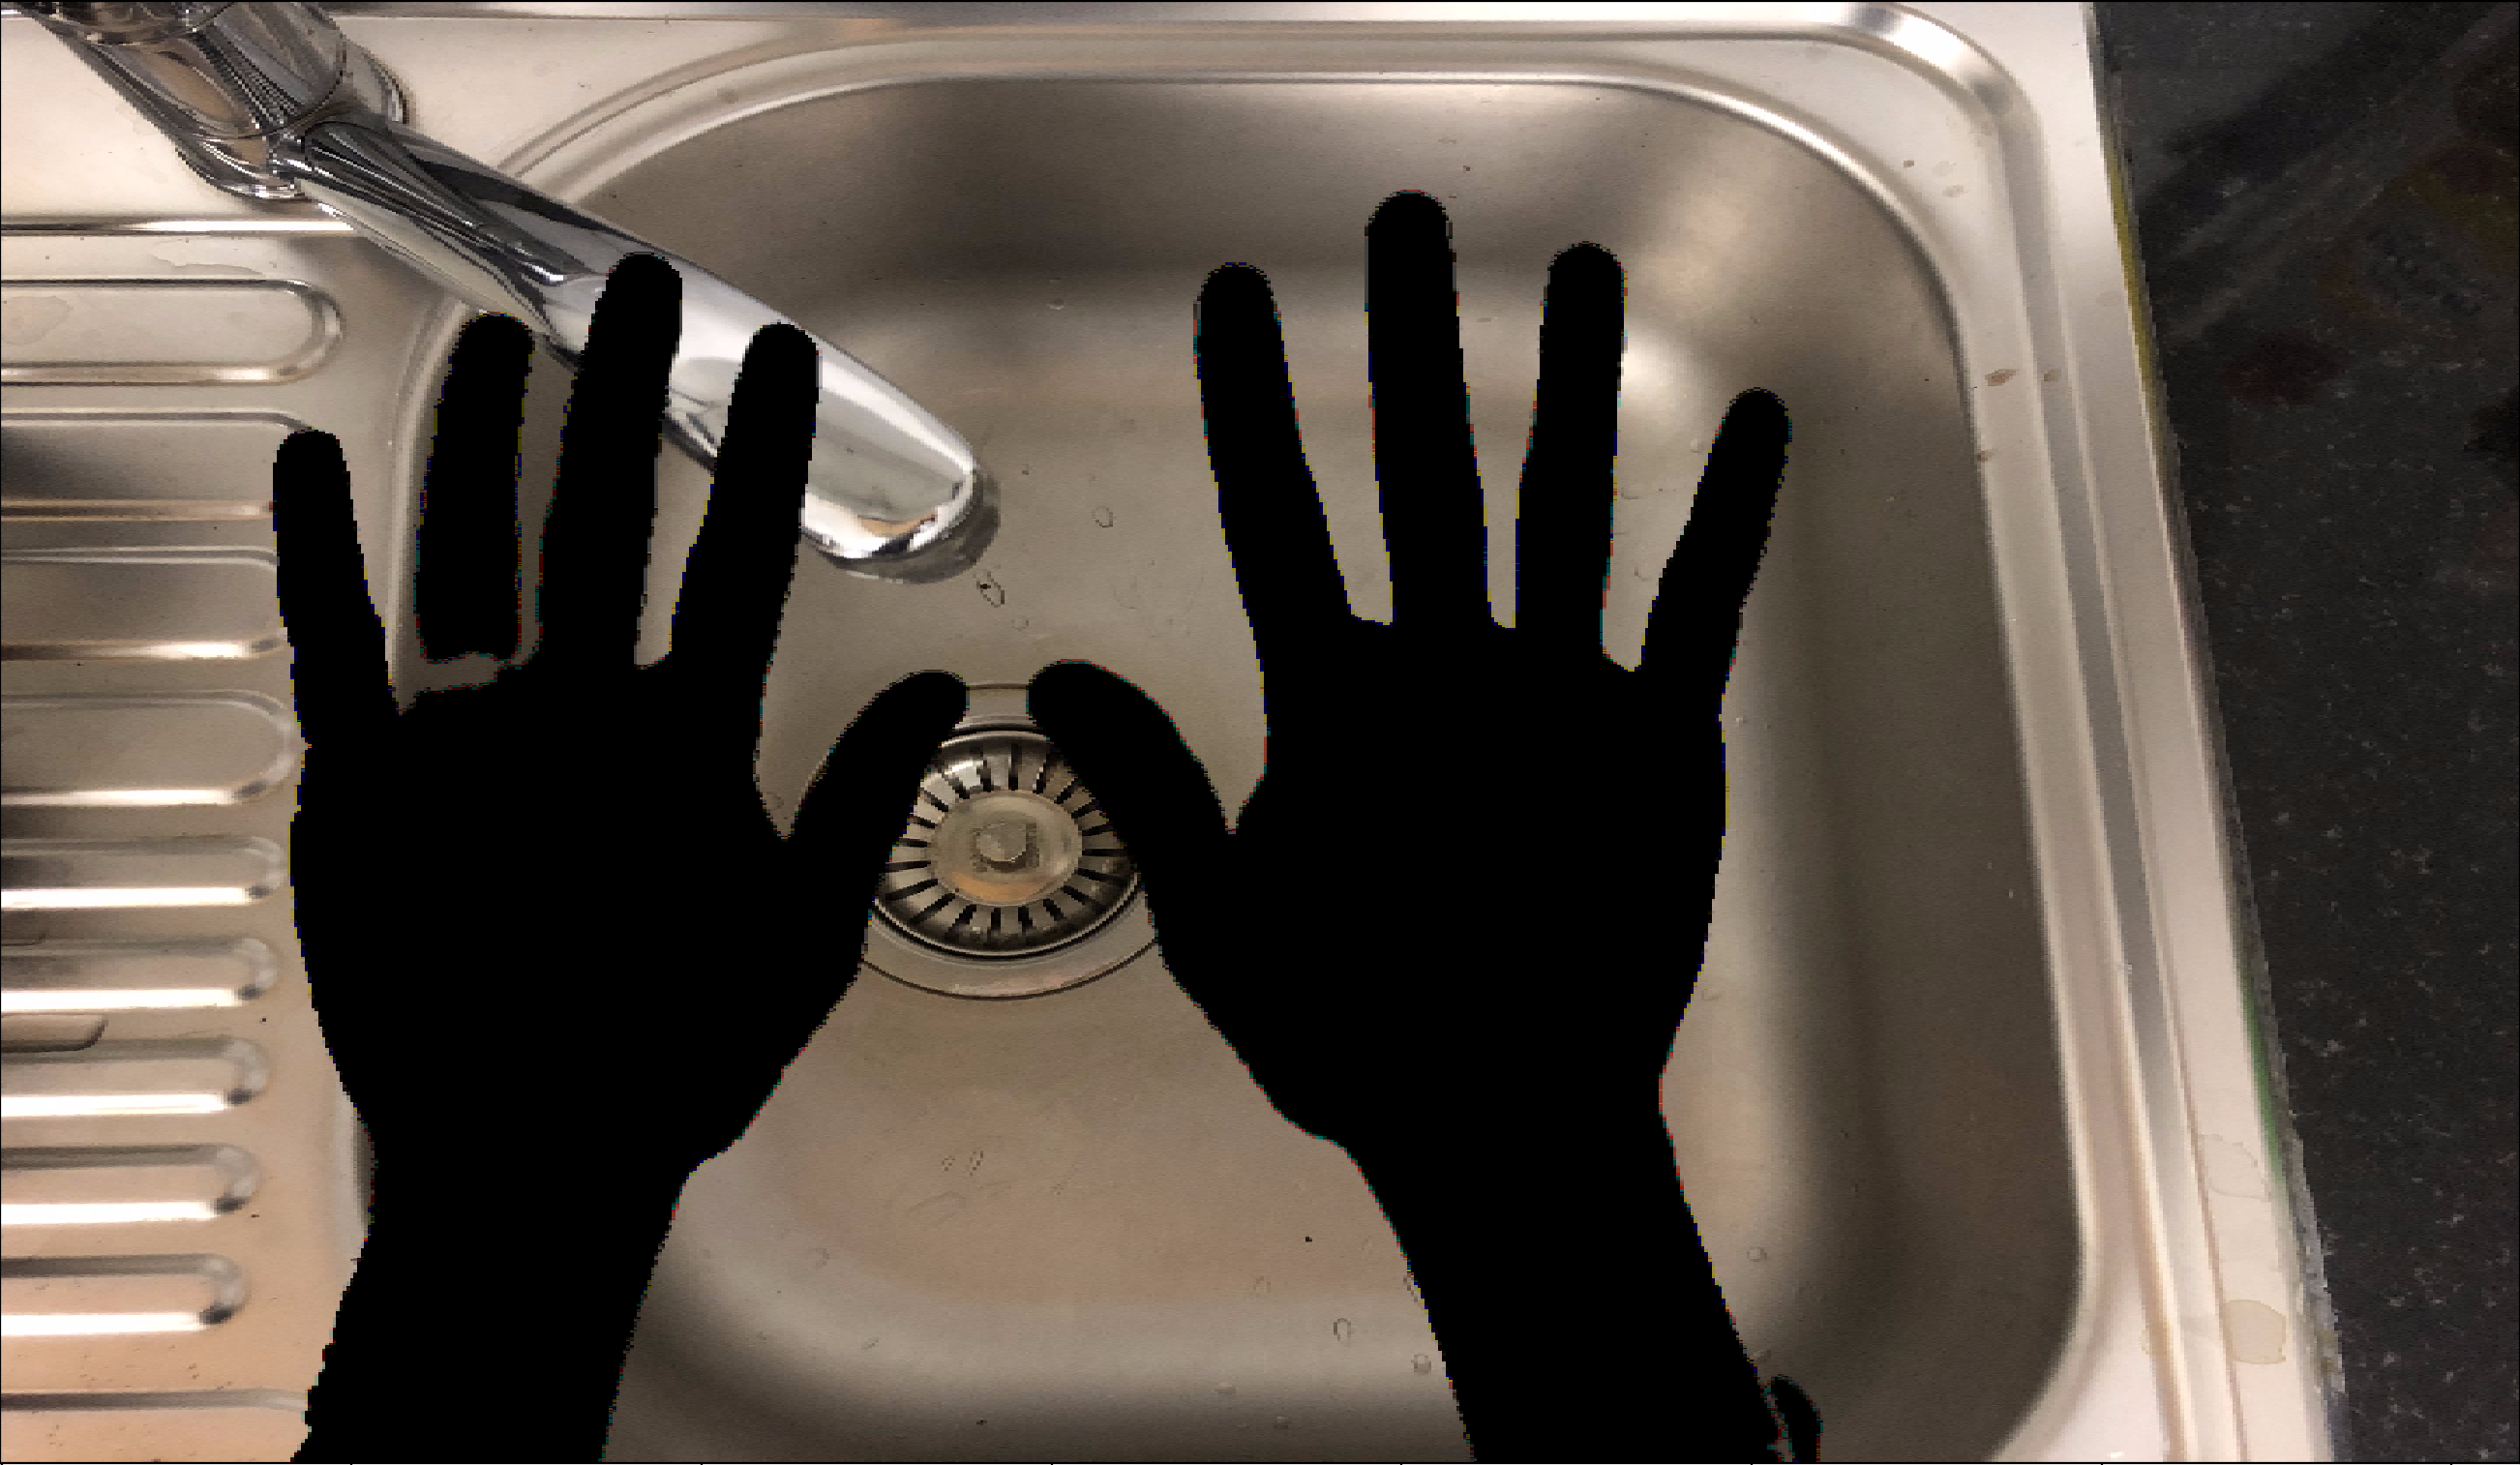
\includegraphics[width=114pt]{../img/handspipeline/5.png}
                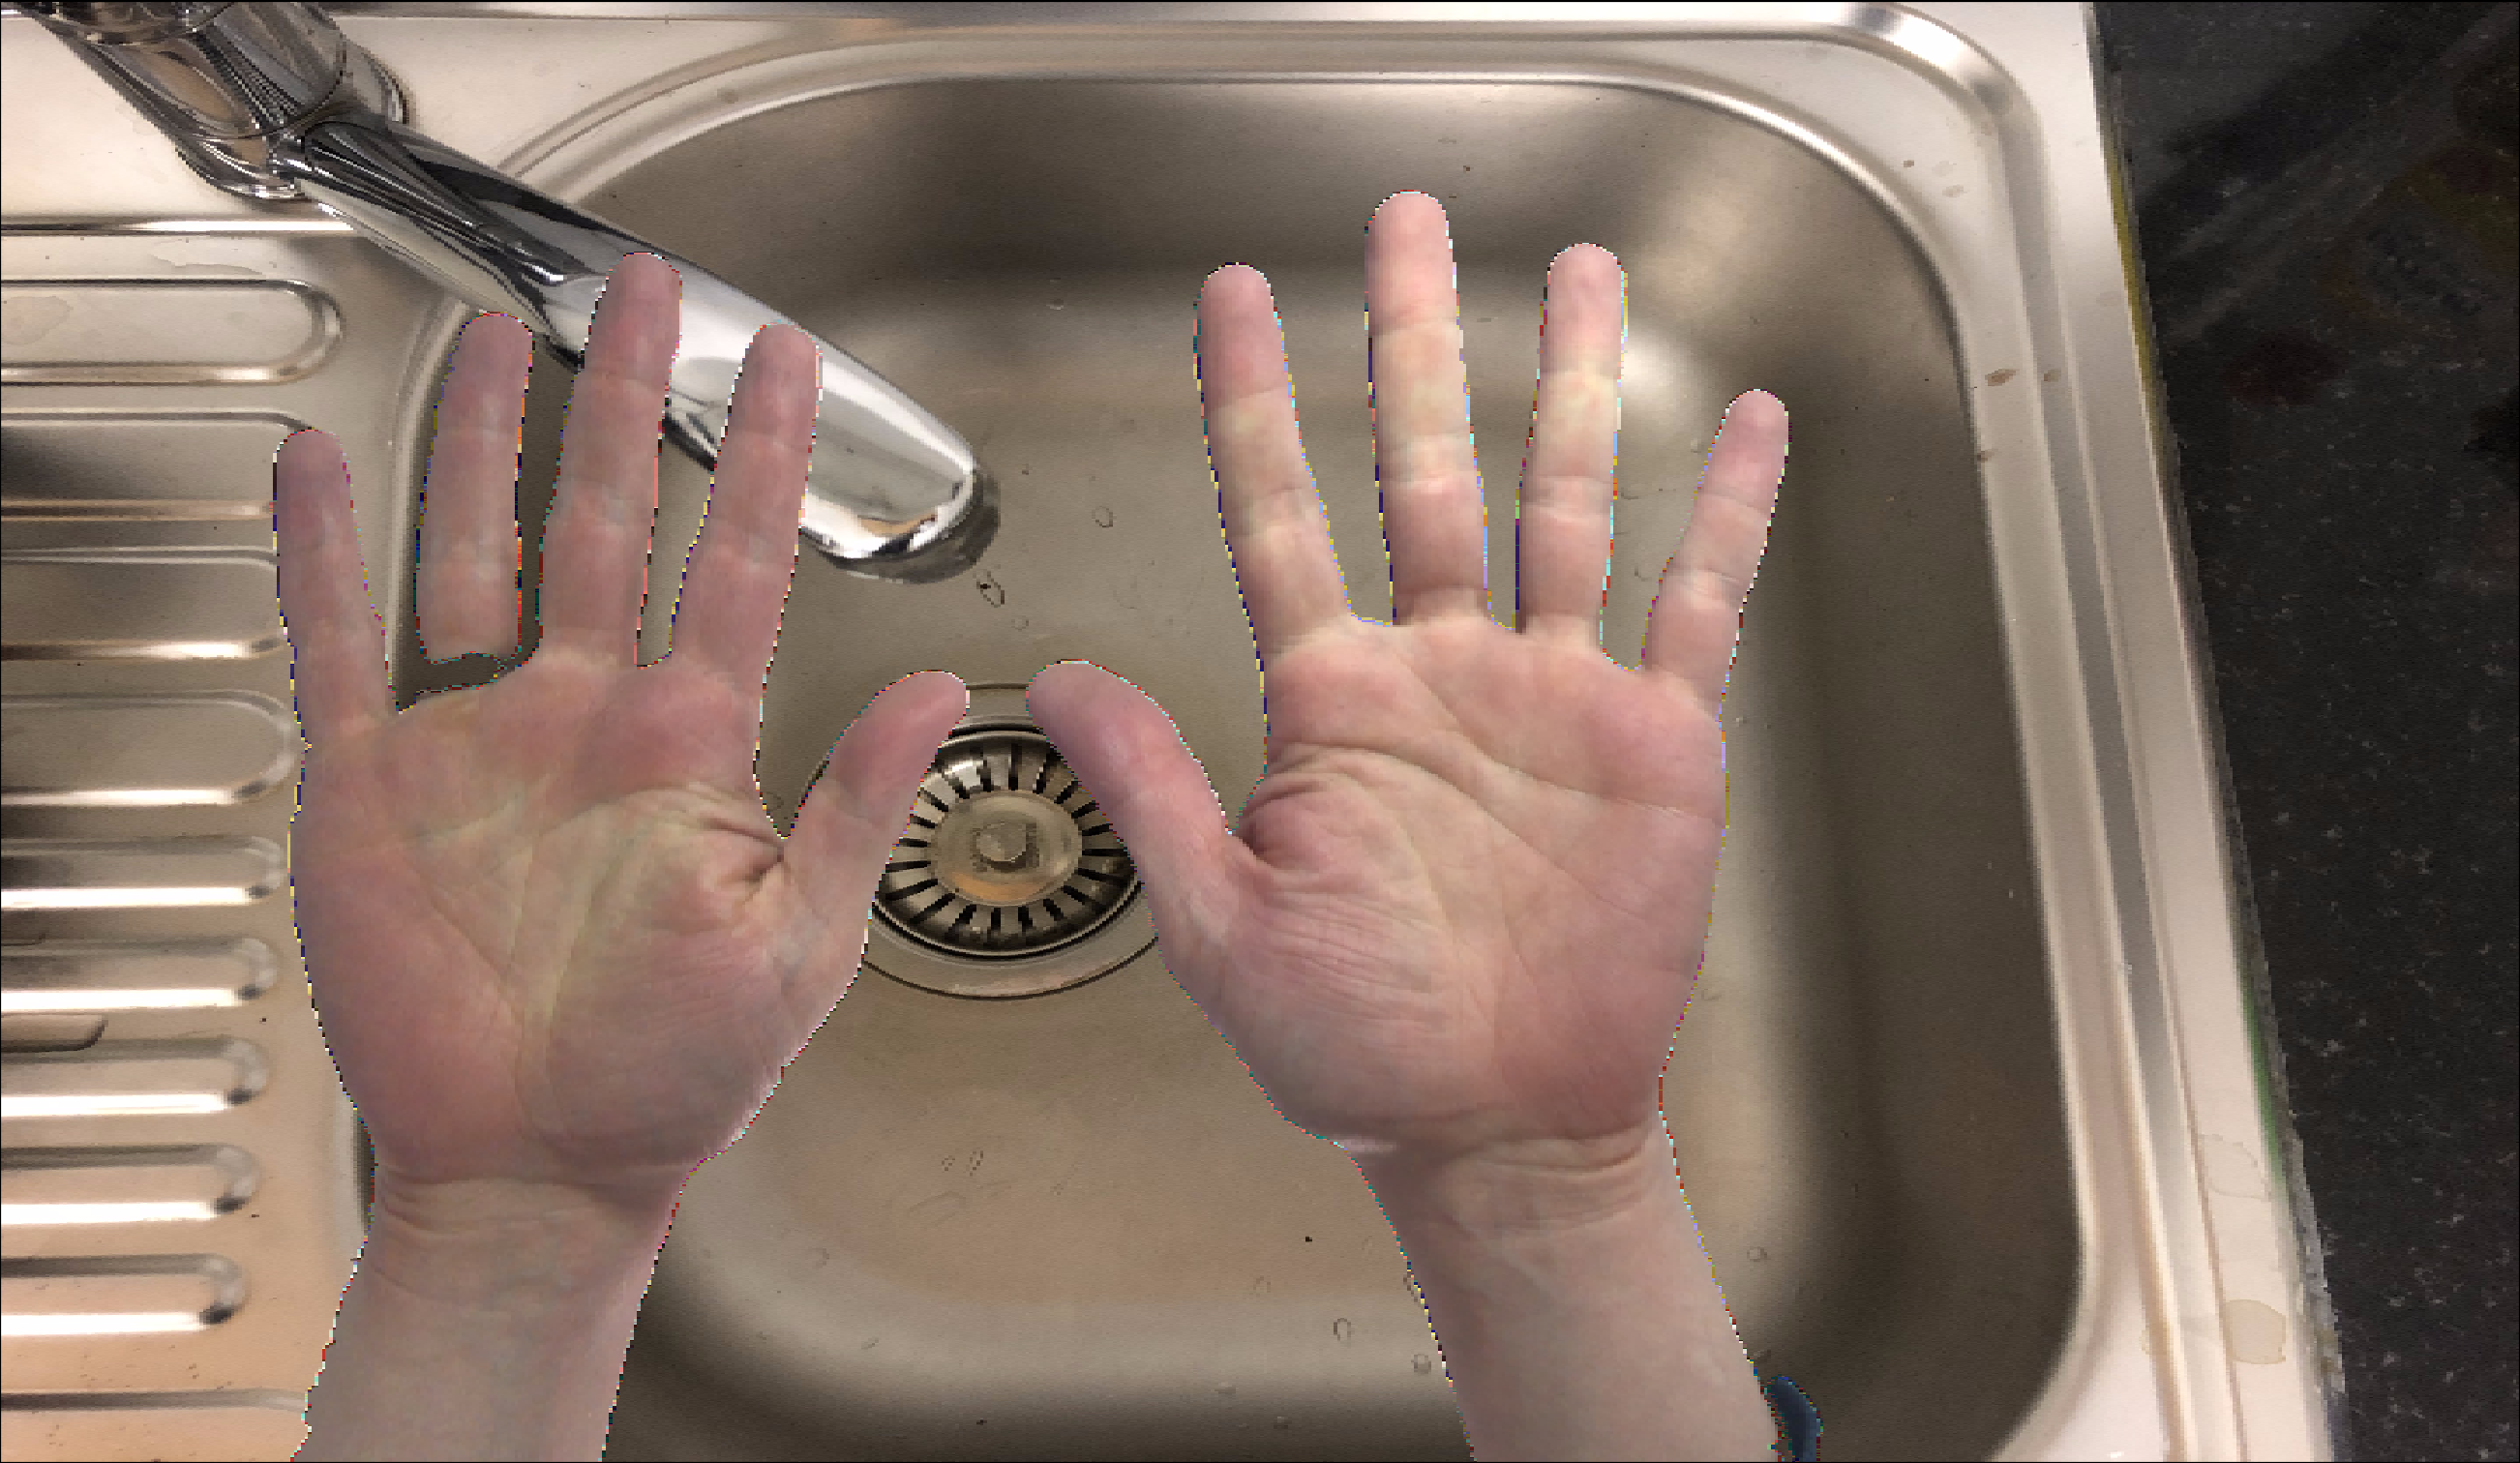
\includegraphics[width=114pt]{../img/handspipeline/6.png}
                \caption{Top left to bottom right: $HAND$, $ROI$, $BACKGROUND$, $Y_{foreground}$, $Y_{background}$, $OUTPUT$. Images \copyright \space Glanta Ltd.}
            \end{figure}

            \subsection{Transformation}
            A transformation can be used as a data augmentation strategy, but some caution needs to be used. As an example, flipping figure \ref{fig:flipped_example} will also change it's class, since there is a corresponding pose for the left and right hands. 

            \begin{figure}[h]
                \centering
                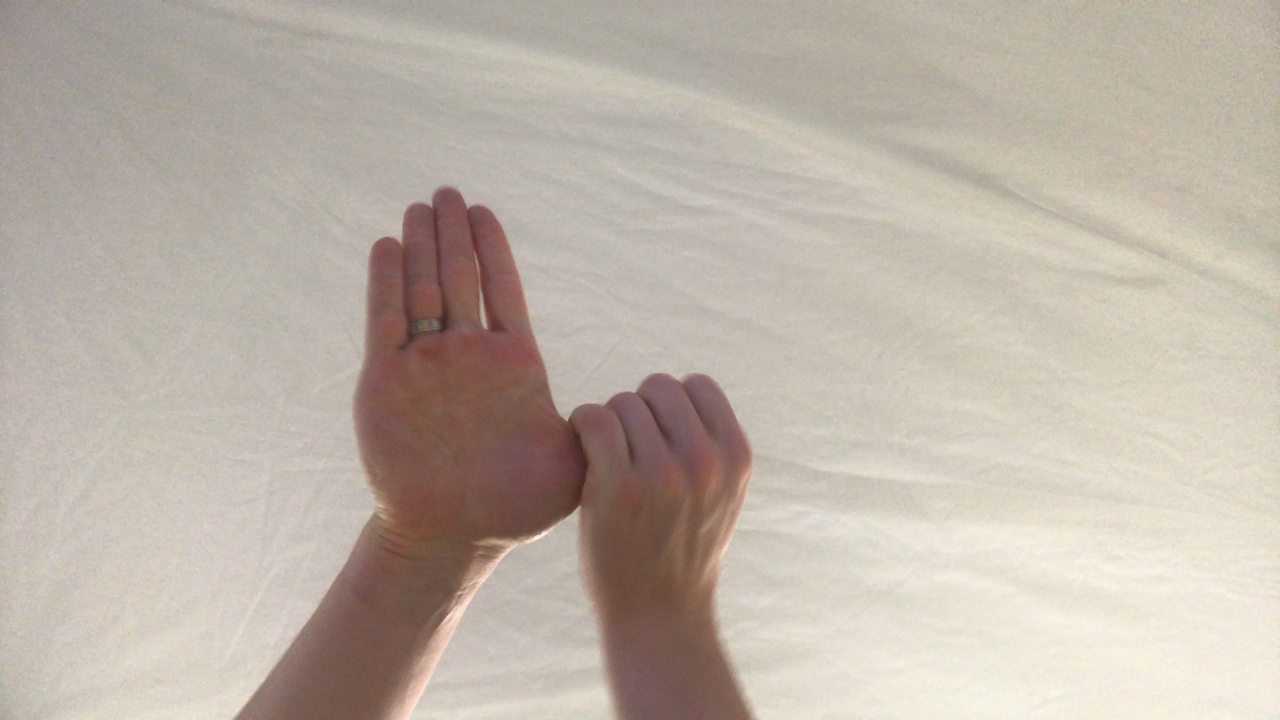
\includegraphics[height=100pt]{../img/flipped_example.png}
                \caption{\copyright \space Glanta Ltd.}
                \label{fig:flipped_example}
            \end{figure}

            
